\documentclass[11pt]{article}
\usepackage{amsmath}
\usepackage{amssymb}
\usepackage{color}
\usepackage{xcolor}
\usepackage{tikz}
\usetikzlibrary{decorations.pathmorphing,decorations.markings}
\tikzset{snake it/.style={decorate, decoration=snake}}

\begin{document}

     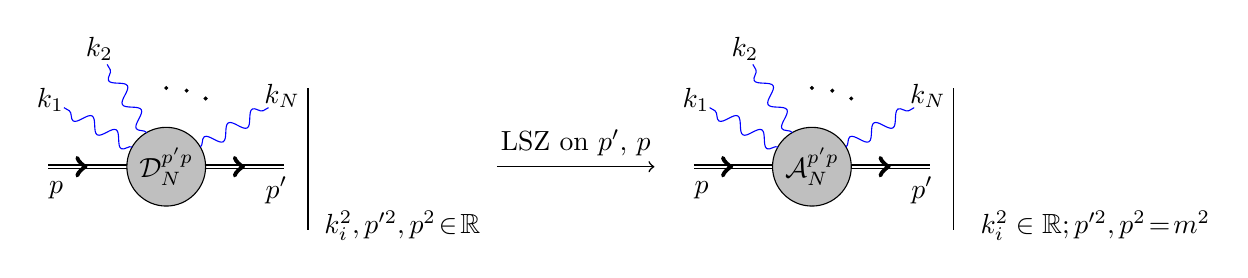
\begin{tikzpicture}
    \begin{scope}[decoration={
    markings,
    mark=at position 0.5 with {\arrow{>}}}
    ] 
            \draw[line width=0.2mm,double,postaction={decorate}] (-1.5,0) -- (-.5,0);
            \draw (-1.4,-.3) node {$p$};
            \draw[line width=0.2mm,double,postaction={decorate}] (.5,0) -- (1.5,0);
            \draw (1.4,-.3) node {$p'$};
            \draw[draw,fill=lightgray] (0,0) circle (0.5) node {$\mathcal{D}^{p'p}_{N}$};
            \draw[draw=blue, snake it] (-0.433013, 0.25) -- (-1.29904, 0.75);
            \draw (-1.47224, 0.85) node {$k_1$};
            \draw[draw=blue, snake it] (-0.25, 0.433013) -- (-0.75, 1.29904);
            \draw (-0.85, 1.5) node {$k_2$};
            \filldraw[black] (0.5, 0.866025) circle (.5pt);
            \filldraw[black] (0.258819, 0.965926) circle (.5pt);
            \filldraw[black] (0, 1) circle (.5pt);
            \draw[draw=blue, snake it] (0.433013, 0.25) -- (1.29904, 0.75);
            \draw (1.47224, 0.9) node {$k_N$};
            \draw (1.8,-.8) --  (1.8,1);
            \draw (3,-.75) node {$k_i^2,p'^2,p^2\!\in\!\mathbb{R}$};
            \draw[line width=0.2mm, ->] (4.2,0) -- (6.2,0);
            \draw (5.2,.3) node {LSZ on $p'$, $p$};
            \draw[line width=0.2mm,double,postaction={decorate}] (-1.5+8.2,0) -- (-.5+8.2,0);
            \draw (-1.4+8.2,-.3) node {$p$};
            \draw[line width=0.2mm,double,postaction={decorate}] (.5+8.2,0) -- (1.5+8.2,0);
            \draw (1.4+8.2,-.3) node {$p'$};
            \draw[draw,fill=lightgray] (8.2,0) circle (0.5) node {$\mathcal{A}^{p'p}_{N}$};
            \draw[draw=blue, snake it] (-0.433013+8.2, 0.25) -- (-1.29904+8.2, 0.75);
            \draw (-1.47224+8.2, 0.85) node {$k_1$};
            \draw[draw=blue, snake it] (-0.25+8.2, 0.433013) -- (-0.75+8.2, 1.29904);
            \draw (-0.85+8.2, 1.5) node {$k_2$};
            \filldraw[black] (0.5+8.2, 0.866025) circle (.5pt);
            \filldraw[black] (0.258819+8.2, 0.965926) circle (.5pt);
            \filldraw[black] (8.2, 1) circle (.5pt);
            \draw[draw=blue, snake it] (0.433013+8.2, 0.25) -- (1.29904+8.2, 0.75);
            \draw (1.47224+8.2, 0.9) node {$k_N$};
            \draw (1.8+8.2,-.8) --  (1.8+8.2,1);
            \draw (3+8.8,-.75) node {$k_i^2\in\mathbb{R};p'^2,p^2\!=\! m^2$};       
        \end{scope}
\end{tikzpicture}

\end{document}